\documentclass[spanish,12pt,letterpapper]{article}
\usepackage{babel}
\usepackage[utf8]{inputenc}
\usepackage{graphicx}
\begin{document}
	\begin{titlepage}
		\begin{center}
			
\includegraphics[width=0.6\textwidth]{./logoUnADM}~\\[1cm] 
			\textsc{Universidad Abierta y a Distancia de México}\\[0.8cm]
			\textsc{Desarrollo de Software}\\[1.8cm]
			
			\textbf{ \Large Actividad 1. Características y ventajas del diseño orientado a objetos }\\[3cm]
			
			Diego Antonio Plascencia Lara\\ ES1421004131 \\[0.4cm]
			Facilitador(a): Rosa Teresa Urvicio Ramirez \\
			Materia: Análisis y diseño orientado a objetos \\
			Grupo: DS-DDOO-1502S-B1-003 \\
			Unidad: I \\
			
			\vfill México D.F\\{\today}
			
		\end{center}
	\end{titlepage}
	
	\part{Caso de análisis y diseño orientado a objetos}
	\section{El caso}
	Para esta actividad trabajare con el caso de un software para una red bancaria, cuya dirección del recurso se encuentra en la sección de Referencias.
	
	\section{Elementos}
	\subsection{Casos de uso} 
	Es el primer elemento en el caso de ejemplo, en este se mencionan en oraciones las diferentes acciones que realiza el usuario, por medio de los casos de uso se puede conocer las razones y módulos a realizar en el sistema, por ejemplo ``El cajero automático envía el número de tarjeta, el código del banco y la contraseña al consorcio.''\\
	
	\subsection{Modelo de objetos.} Consta de diferentes pasos los cuales son:
	\paragraph{Identificar objetos y clases.} 
	\subparagraph{Se seleccionan los nombres en los requisitos:} ``Software, Red bancaria, Cajero automático...''.
	\subparagraph{Se añaden clases adicionales, procedentes de nuestro conocimiento de tema:} ``Podemos añadir la clase Línea de comunicaciones.''
	\subparagraph{Eliminar  redundancias:} ``Cliente y Usuario son la misma clase. Nos quedamos con Cliente por adaptarse mejor al concepto.''
	\subparagraph{Eliminar clases irrelevantes:} ``Coste de desarrollo no tiene nada que ver con el problema, queda fuera del sistema.''
	\subparagraph{Eliminar clases vagas:}``Sistema, Características de seguridad, Red bancaria y Parte compartida pueden considerarse vagas.''
	\subparagraph{Separar atributos:}``Los atributos definen datos asociados a un objeto, en lugar de objetos. Aunque la separación no es clara (los atributos pueden ser objetos embebidos) en algunos casos se pueden distinguir. En el ejemplo, pueden considerarse atributos Información sobre la cuenta, (atributo de Cuenta bancaria), Dinero en efectivo y Recibo (atributos de Cajero automático).''
	\subparagraph{Separar métodos:}``Algunos nombres (por ejemplo, Llamada telefónica) definen realmente operaciones o eventos.''
	\subparagraph{Eliminar objetos de diseño:}``Todas las clases que corresponden más a la solución del problema que a la situación real, deben considerarse objetos de diseño y eliminarse en la fase del análisis. En el ejemplo, eliminaremos Registro de transacciones, Línea de comunicaciones, Acceso a la cuenta y Software.''
	
	\paragraph{Identificar y depurar relaciones.}
	\subparagraph{Seleccionar verbos relacionales en los requisitos:} ``Las Estaciones de cajero están conectadas al Ordenador del banco.''
	\subparagraph{Añadir relaciones adicionales procedentes de nuestro conocimiento del tema:} ``Las Tarjetas de crédito están asociadas a las Cuentas bancarias .''
	\subparagraph{Eliminar relaciones de diseño o entre clases eliminadas:} ``Una Red bancaria está provista de Cajeros automáticos.''
	\subparagraph{Eliminar eventos transitorios:} ``Los Cajeros automáticos interaccionan con el Usuario.''
	\subparagraph{Reducir relaciones ternarias:}``a. El Cajero humano introduce Transacciones, b. Las Transacciones actúan sobre las Cuentas bancarias.''
	\subparagraph{Eliminar relaciones redundantes o derivadas:}``Los Cajeros automáticos comunican con el Ordenador central.''
	\subparagraph{Añadir relaciones olvidadas:}``Los Clientes tienen Cuentas.''
	\subparagraph{Definir la multiplicidad de cada relación:}``Un Cliente puede tener muchas Tarjetas de crédito.''
	
	\paragraph{Identificar atributos de objetos y relaciones.}
	\subparagraph{Atributos de los objetos:}``De la Cuenta: Saldo, Límite de crédito, Tipo de cuenta.''
	\subparagraph{Atributos de las relaciones:}``Código de la estación de cajero.''
	
	\paragraph{Añadir herencia.}``La clase Estación de entrada será superclase de Cajero automático y de Estación de cajero.''
	
	\paragraph{Comprobar los casos de uso (iterar).} ``Tarjeta de crédito desempeña dos roles: la tarjeta física, que se introduce y que permite al cajero automático conectarse con el banco, con información sobre el mundo real (banco, número de la tarjeta) y las autorizaciones concedidas por éste, que sólo son números en la memoria de un ordenador y se pueden cambiar con facilidad (contraseña, límite de crédito). Se puede descomponer en Tarjeta de crédito y Autorización de la tarjeta. Una sola autorización puede afectar a más de una tarjeta física. Una misma autorización puede permitir acceder a más de una cuenta (y viceversa).''
	
	\paragraph{Modularizar.} ``Cuentas en general: Cuenta, Tarjeta de crédito, Autorización, Cliente, Transacción, Transacción de cajero, Transacción remota.''
	
	\paragraph{Añadir y simplificar métodos.} ``Añadir métodos que permitan navegar de un objeto a otro.''\\
	
	\subsection{Modelo dinámico}
	consta de los siguientes pasos:
	
	\paragraph{Identificar sucesos.} Resultados: Diagramas de secuencia (trazas de eventos) y diagramas de colaboración (diagramas de flujo de eventos). Los casos de uso (escenarios) se convierten en diagramas de secuencia. Estas se compactan en diagramas de colaboración
	
	\paragraph{Construir diagramas de estados.} Uno por clase. En el ejemplo de los cajeros automáticos deben centrarse en las clases dinámicas, que cambian de estado.
	
	\paragraph{Añadir métodos.} Los eventos son métodos. Es preciso decidir de qué clase de objetos. Las acciones y actividades realizadas en los estados son métodos.\\
	
	\subsection{Modelo funcional.}
	
	\paragraph{Identificar valores de entrada/salida.} Son los que pasan información desde los objetos externos al sistema de software propiamente dicho.
	\paragraph{Construir diagramas de flujo de actividad.} Relacionan los valores de entrada con los de salida. Suele dividirse en varias capas o niveles.
	\paragraph{Describir funciones.} Descripción de cada una de las funciones de nivel mínimo que aparecen en los diagramas de flujo de actividad
		\paragraph{Identificar restricciones y dependencias funcionales entre objetos.}``El saldo de una cuenta no puede ser negativo''
	\paragraph{Definir criterios de optimización (iterar).} ``Minimizar el número de mensajes enviados entre localidades diferentes.''
	\paragraph{Añadir métodos.} Las funciones del modelo funcional pueden ser simples transferencias de información, o corresponder a un método de algún objeto (operaciones interesantes). En este caso hay que asignarlos y añadirlos al modelo de objetos.\\
	
	\section{Descripción e Interés}
	Este ejemplo de análisis orientado a objetos es sobre una red bancaria, en donde se toma en cuenta todo proceso interno y externo de un ATM o cajero, donde se involucra la lógica de la interfaz con la que interactúan el usuario y todo aquello que es propio de las operaciones bancarias internas.\\
	
	Me intereso este ejemplo por que aunque sea un típico caso, es el que muestra en mayor amplitud algo cercano a todo el proceso de análisis orientado objetos, puesto que es algo común, que debe ser sencillo al tratarse de la parte de la interfaz, pero elaborado por tratarse de un banco.
	
	\pagebreak
	\part{Replanteamiento en situación personal}
	\section{Caso de un punto de venta para una tortillería}
	Un caso personal es el de un negocio familiar que apenas va empezando y que me gustaría darle un impulso con ayuda de la tecnología, por lo que para este replanteamiento me enfocare en un pequeño punto de venta para dispositivo móvil que tan solo ayude a llevar el historial de ventas y a hacer la información de pagos.
	\subsection{Casos de uso}
	\begin{itemize}
		\item El cliente pide el producto que necesita (tortillas, comida). 
		\item El cliente pide una cantidad de ``tupper'' (comida).
		\item El cliente pide tortillas en KG o precio.
		\item El trabajador debe ingresar la cantidad de producto de la venta en el PDV.
		\item El PDV recive la cantidad de producto que se vende.
		\item El PDV muestra el total de la venta.
		\item El trabajador debe proporcionar el tupper solicitado.
		\item El trabajador debe proporcionar la cantidad de tortillas solicitadas.
		\item El trabajador debe indicar al cliente el total de la venta.
		\item El cliente proporciona el dinero al trabajador.
		\item El trabajador recibe el dinero del cliente.
		\item El trabajador debe ingresar en el PDV la cantidad de dinero recibida por el cliente.
		\item El PDV recibe la cantidad de dinero recibida por el cliente.
		\item El PDV muestra el cambio que debe regresarsele al cliente.
		\item El PDV registra en el historial de ventas la información de la venta.
		\item El trabajador proporciona el cambio al cliente.\\
	\end{itemize}
	
	\subsection{Modelado}
	Para esta sección unicamente haría uso de 3 Interfaces, y 5 clases, de las cuales 2 extienden:
	\begin{itemize}
		\item (interface) PointOfSale
		\item (interface) Product
		\item (interface) Sale
		\item (implemented Class) TortilleriaSale
		\item (implemented Class) TortilleriaPointOfSale
		\item (implemented Class) TortilleriaProduct
		\item (extended Class) CountableProduct
		\item (extended Class) WeighableProduct \pagebreak
	\end{itemize}
	
	\begin{center}
		Este es un posible diagrama de como podría quedar el modelo: \\[1cm]
		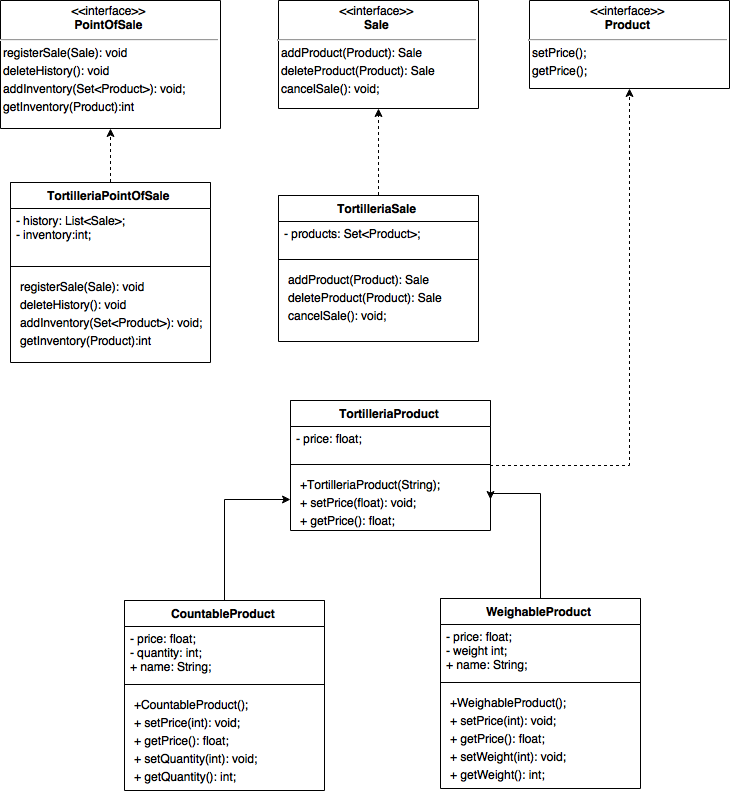
\includegraphics[width=0.6\textwidth]{./OODiagram}~\\[1cm]
	\end{center}

	
	
	\section{Diferencia entre analisis, diseño y programación orientada a objetos}
	
	La diferencia esta en que el análisis es el preámbulo de la programación, es decir que el análisis trata de recabar todos los requerimientos, los casos de uso, utilizar diagramas u otras herramientas para modelar todo lo necesario para poder analizar estos datos y requerimientos.\\
	
	Mientras que el diseño o programación, es aplicar todo lo recabado en el análisis, y hacer la programación con algún lenguaje orientado a objetos siguiendo los requerimientos necesarios.
	
	\pagebreak
	\begin{thebibliography}{9}
		\bibitem{casoAOO} Escuela Politécnica Superior.
		\emph{Ejemplo de Análisis Orientado a Objetos} {[} En linea {]}, España. Disponible en: \textgreater http://arantxa.ii.uam.es/~alfonsec/atm.htm \textless
	\end{thebibliography}
\end{document}